\documentclass[twoside]{book}

% Packages required by doxygen
\usepackage{fixltx2e}
\usepackage{calc}
\usepackage{doxygen}
\usepackage[export]{adjustbox} % also loads graphicx
\usepackage{graphicx}
\usepackage[utf8]{inputenc}
\usepackage{makeidx}
\usepackage{multicol}
\usepackage{multirow}
\PassOptionsToPackage{warn}{textcomp}
\usepackage{textcomp}
\usepackage[nointegrals]{wasysym}
\usepackage[table]{xcolor}

% NLS support packages
\usepackage[T2A]{fontenc}
\usepackage[russian]{babel}

% Font selection
\usepackage[T1]{fontenc}
\usepackage[scaled=.90]{helvet}
\usepackage{courier}
\usepackage{amssymb}
\usepackage{sectsty}
\renewcommand{\familydefault}{\sfdefault}
\allsectionsfont{%
  \fontseries{bc}\selectfont%
  \color{darkgray}%
}
\renewcommand{\DoxyLabelFont}{%
  \fontseries{bc}\selectfont%
  \color{darkgray}%
}
\newcommand{\+}{\discretionary{\mbox{\scriptsize$\hookleftarrow$}}{}{}}

% Page & text layout
\usepackage{geometry}
\geometry{%
  a4paper,%
  top=2.5cm,%
  bottom=2.5cm,%
  left=2.5cm,%
  right=2.5cm%
}
\tolerance=750
\hfuzz=15pt
\hbadness=750
\setlength{\emergencystretch}{15pt}
\setlength{\parindent}{0cm}
\setlength{\parskip}{0.2cm}
\makeatletter
\renewcommand{\paragraph}{%
  \@startsection{paragraph}{4}{0ex}{-1.0ex}{1.0ex}{%
    \normalfont\normalsize\bfseries\SS@parafont%
  }%
}
\renewcommand{\subparagraph}{%
  \@startsection{subparagraph}{5}{0ex}{-1.0ex}{1.0ex}{%
    \normalfont\normalsize\bfseries\SS@subparafont%
  }%
}
\makeatother

% Headers & footers
\usepackage{fancyhdr}
\pagestyle{fancyplain}
\fancyhead[LE]{\fancyplain{}{\bfseries\thepage}}
\fancyhead[CE]{\fancyplain{}{}}
\fancyhead[RE]{\fancyplain{}{\bfseries\leftmark}}
\fancyhead[LO]{\fancyplain{}{\bfseries\rightmark}}
\fancyhead[CO]{\fancyplain{}{}}
\fancyhead[RO]{\fancyplain{}{\bfseries\thepage}}
\fancyfoot[LE]{\fancyplain{}{}}
\fancyfoot[CE]{\fancyplain{}{}}
\fancyfoot[RE]{\fancyplain{}{\bfseries\scriptsize Документация по Template. Последние изменения\+: Пт 29 Май 2015 15\+:57\+:07. Создано системой Doxygen }}
\fancyfoot[LO]{\fancyplain{}{\bfseries\scriptsize Документация по Template. Последние изменения\+: Пт 29 Май 2015 15\+:57\+:07. Создано системой Doxygen }}
\fancyfoot[CO]{\fancyplain{}{}}
\fancyfoot[RO]{\fancyplain{}{}}
\renewcommand{\footrulewidth}{0.4pt}
\renewcommand{\chaptermark}[1]{%
  \markboth{#1}{}%
}
\renewcommand{\sectionmark}[1]{%
  \markright{\thesection\ #1}%
}

% Indices & bibliography
\usepackage{natbib}
\usepackage[titles]{tocloft}
\setcounter{tocdepth}{3}
\setcounter{secnumdepth}{5}
\makeindex

% Hyperlinks (required, but should be loaded last)
\usepackage{ifpdf}
\ifpdf
  \usepackage[pdftex,pagebackref=true]{hyperref}
\else
  \usepackage[ps2pdf,pagebackref=true]{hyperref}
\fi
\hypersetup{%
  colorlinks=true,%
  linkcolor=blue,%
  citecolor=blue,%
  unicode%
}

% Custom commands
\newcommand{\clearemptydoublepage}{%
  \newpage{\pagestyle{empty}\cleardoublepage}%
}


%===== C O N T E N T S =====

\begin{document}

% Titlepage & ToC
\hypersetup{pageanchor=false,
             bookmarks=true,
             bookmarksnumbered=true,
             pdfencoding=unicode
            }
\pagenumbering{roman}
\begin{titlepage}
\vspace*{7cm}
\begin{center}%
{\Large Template }\\
\vspace*{1cm}
{\large Создано системой Doxygen 1.8.9.1}\\
\vspace*{0.5cm}
{\small Пт 29 Май 2015 15:57:07}\\
\end{center}
\end{titlepage}
\clearemptydoublepage
\tableofcontents
\clearemptydoublepage
\pagenumbering{arabic}
\hypersetup{pageanchor=true}

%--- Begin generated contents ---
\chapter{Иерархический список классов}
\section{Иерархия классов}
Иерархия классов.\begin{DoxyCompactList}
\item \contentsline{section}{Spisok$<$ T $>$}{\pageref{struct_spisok}}{}
\begin{DoxyCompactList}
\item \contentsline{section}{S\+Spisok$<$ T $>$}{\pageref{class_s_spisok}}{}
\end{DoxyCompactList}
\end{DoxyCompactList}

\chapter{Алфавитный указатель классов}
\section{Классы}
Классы с их кратким описанием.\begin{DoxyCompactList}
\item\contentsline{section}{\hyperlink{struct_spisok}{Spisok$<$ T $>$} \\*Шаблоны (англ. template) — средство языка C++, предназначенное для кодирования обобщённых алгоритмов, без привязки к некоторым параметрам (например, типам данных, размерам буферов, значениям по умолчанию) }{\pageref{struct_spisok}}{}
\item\contentsline{section}{\hyperlink{class_s_spisok}{S\+Spisok$<$ T $>$} }{\pageref{class_s_spisok}}{}
\end{DoxyCompactList}

\chapter{Список файлов}
\section{Файлы}
Полный список файлов.\begin{DoxyCompactList}
\item\contentsline{section}{T\+I\+M\+P\+Shablon/\hyperlink{1212_8cpp}{1212.\+cpp} }{\pageref{1212_8cpp}}{}
\end{DoxyCompactList}

\chapter{Классы}
\hypertarget{struct_spisok}{}\section{Шаблон структуры Spisok$<$ T $>$}
\label{struct_spisok}\index{Spisok$<$ T $>$@{Spisok$<$ T $>$}}


Шаблоны (англ. template) — средство языка C++, предназначенное для кодирования обобщённых алгоритмов, без привязки к некоторым параметрам (например, типам данных, размерам буферов, значениям по умолчанию).  


Граф наследования\+:Spisok$<$ T $>$\+:\begin{figure}[H]
\begin{center}
\leavevmode
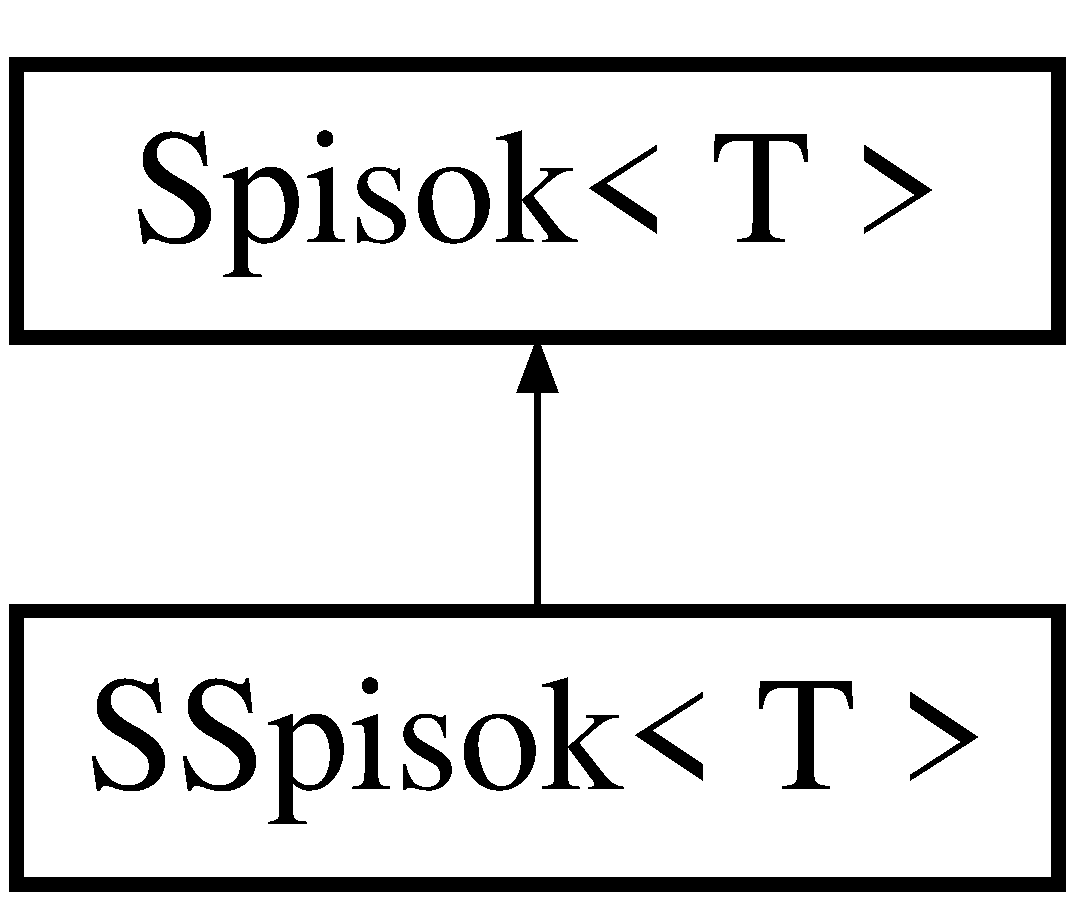
\includegraphics[height=2.000000cm]{struct_spisok}
\end{center}
\end{figure}
\subsection*{Открытые атрибуты}
\begin{DoxyCompactItemize}
\item 
T \hyperlink{struct_spisok_aa25d518a0e44cdd1c882051db5af9e04}{data}
\begin{DoxyCompactList}\small\item\em data -\/ информационное поле \end{DoxyCompactList}\item 
\hyperlink{struct_spisok}{Spisok} $\ast$ \hyperlink{struct_spisok_a55a474ff28ffad84e395d7a481717832}{next}
\begin{DoxyCompactList}\small\item\em $\ast$next -\/ указатель на следующий элемент \end{DoxyCompactList}\item 
\hyperlink{struct_spisok}{Spisok} $\ast$ \hyperlink{struct_spisok_a5898c0910b43a9c6e55224bb5fd89416}{pred}
\begin{DoxyCompactList}\small\item\em $\ast$pred -\/ указатель на предыдуший элемент \end{DoxyCompactList}\end{DoxyCompactItemize}


\subsection{Подробное описание}
\subsubsection*{template$<$class T$>$struct Spisok$<$ T $>$}

Шаблоны (англ. template) — средство языка C++, предназначенное для кодирования обобщённых алгоритмов, без привязки к некоторым параметрам (например, типам данных, размерам буферов, значениям по умолчанию). 

\subsection{Данные класса}
\hypertarget{struct_spisok_aa25d518a0e44cdd1c882051db5af9e04}{}\index{Spisok@{Spisok}!data@{data}}
\index{data@{data}!Spisok@{Spisok}}
\subsubsection[{data}]{\setlength{\rightskip}{0pt plus 5cm}template$<$class T $>$ T {\bf Spisok}$<$ T $>$\+::data}\label{struct_spisok_aa25d518a0e44cdd1c882051db5af9e04}


data -\/ информационное поле 

\hypertarget{struct_spisok_a55a474ff28ffad84e395d7a481717832}{}\index{Spisok@{Spisok}!next@{next}}
\index{next@{next}!Spisok@{Spisok}}
\subsubsection[{next}]{\setlength{\rightskip}{0pt plus 5cm}template$<$class T $>$ {\bf Spisok}$\ast$ {\bf Spisok}$<$ T $>$\+::next}\label{struct_spisok_a55a474ff28ffad84e395d7a481717832}


$\ast$next -\/ указатель на следующий элемент 

\hypertarget{struct_spisok_a5898c0910b43a9c6e55224bb5fd89416}{}\index{Spisok@{Spisok}!pred@{pred}}
\index{pred@{pred}!Spisok@{Spisok}}
\subsubsection[{pred}]{\setlength{\rightskip}{0pt plus 5cm}template$<$class T $>$ {\bf Spisok}$\ast$ {\bf Spisok}$<$ T $>$\+::pred}\label{struct_spisok_a5898c0910b43a9c6e55224bb5fd89416}


$\ast$pred -\/ указатель на предыдуший элемент 



Объявления и описания членов структуры находятся в файле\+:\begin{DoxyCompactItemize}
\item 
T\+I\+M\+P\+Shablon/\hyperlink{1212_8cpp}{1212.\+cpp}\end{DoxyCompactItemize}

\hypertarget{class_s_spisok}{}\section{Шаблон класса S\+Spisok$<$ T $>$}
\label{class_s_spisok}\index{S\+Spisok$<$ T $>$@{S\+Spisok$<$ T $>$}}
Граф наследования\+:S\+Spisok$<$ T $>$\+:\begin{figure}[H]
\begin{center}
\leavevmode
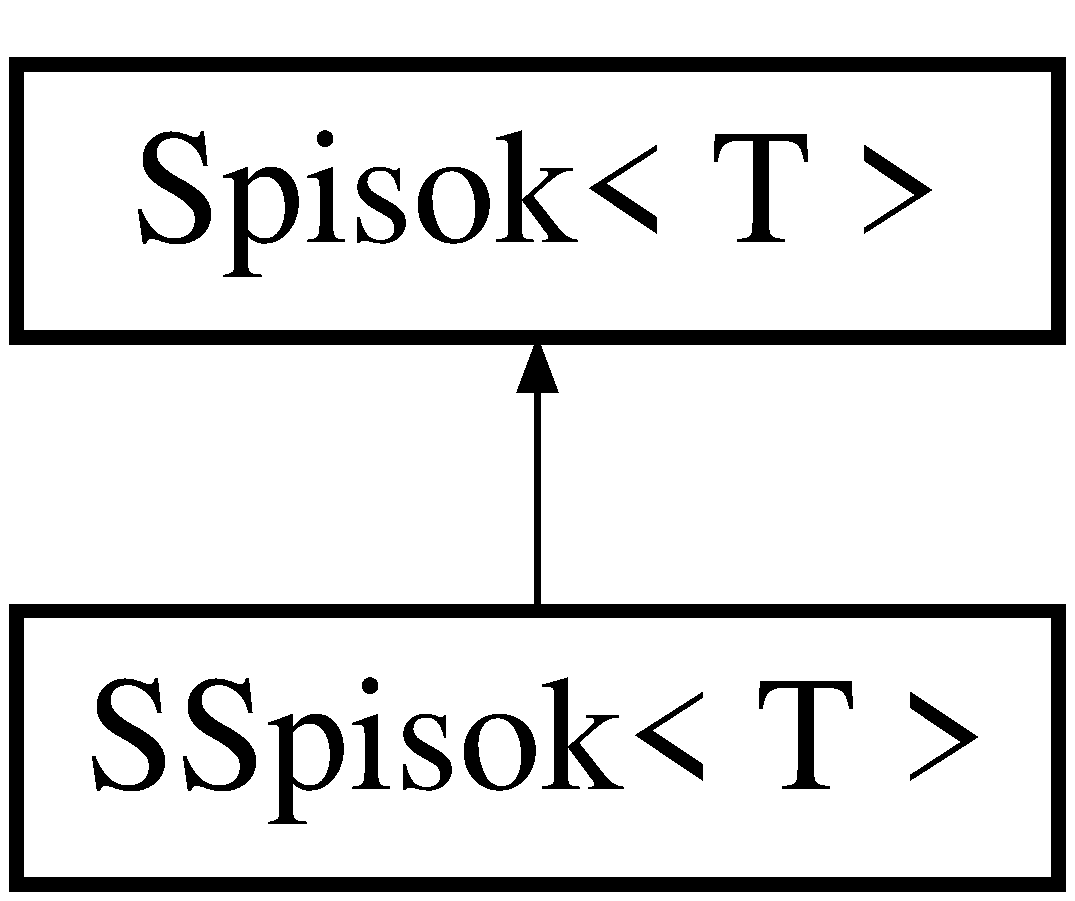
\includegraphics[height=2.000000cm]{class_s_spisok}
\end{center}
\end{figure}
\subsection*{Открытые члены}
\begin{DoxyCompactItemize}
\item 
\hyperlink{class_s_spisok_a3a0baf65e6ad74d1724a96ad2960033e}{S\+Spisok} ()
\item 
void \hyperlink{class_s_spisok_a903c34a2eca29dd44589ce8f9aae22f5}{Add\+Spisok} (int position, T value)
\item 
void \hyperlink{class_s_spisok_a6fe2f4f11b4b4ecdebde6897c6d236d8}{Print\+Spisok} ()
\end{DoxyCompactItemize}
\subsection*{Дополнительные унаследованные члены}


\subsection{Конструктор(ы)}
\hypertarget{class_s_spisok_a3a0baf65e6ad74d1724a96ad2960033e}{}\index{S\+Spisok@{S\+Spisok}!S\+Spisok@{S\+Spisok}}
\index{S\+Spisok@{S\+Spisok}!S\+Spisok@{S\+Spisok}}
\subsubsection[{S\+Spisok}]{\setlength{\rightskip}{0pt plus 5cm}template$<$class T $>$ {\bf S\+Spisok}$<$ T $>$\+::{\bf S\+Spisok} (
\begin{DoxyParamCaption}
{}
\end{DoxyParamCaption}
)\hspace{0.3cm}{\ttfamily [inline]}}\label{class_s_spisok_a3a0baf65e6ad74d1724a96ad2960033e}


\subsection{Методы}
\hypertarget{class_s_spisok_a903c34a2eca29dd44589ce8f9aae22f5}{}\index{S\+Spisok@{S\+Spisok}!Add\+Spisok@{Add\+Spisok}}
\index{Add\+Spisok@{Add\+Spisok}!S\+Spisok@{S\+Spisok}}
\subsubsection[{Add\+Spisok}]{\setlength{\rightskip}{0pt plus 5cm}template$<$class T $>$ void {\bf S\+Spisok}$<$ T $>$\+::Add\+Spisok (
\begin{DoxyParamCaption}
\item[{int}]{position, }
\item[{T}]{value}
\end{DoxyParamCaption}
)}\label{class_s_spisok_a903c34a2eca29dd44589ce8f9aae22f5}
Функция добавления элемента Spisok$<$\+T$>$ $\ast$node=new Spisok$<$\+T$>$ создание нового элемента

node-\/$>$data=value присвоение элементу значения

if (head==N\+U\+L\+L) если список пуст

node-\/$>$next=node установка указателя next

node-\/$>$pred=node установка указателя prev

определяется голова списка

node-\/$>$next=p добавление элемента \hypertarget{class_s_spisok_a6fe2f4f11b4b4ecdebde6897c6d236d8}{}\index{S\+Spisok@{S\+Spisok}!Print\+Spisok@{Print\+Spisok}}
\index{Print\+Spisok@{Print\+Spisok}!S\+Spisok@{S\+Spisok}}
\subsubsection[{Print\+Spisok}]{\setlength{\rightskip}{0pt plus 5cm}template$<$class T $>$ void {\bf S\+Spisok}$<$ T $>$\+::Print\+Spisok (
\begin{DoxyParamCaption}
{}
\end{DoxyParamCaption}
)}\label{class_s_spisok_a6fe2f4f11b4b4ecdebde6897c6d236d8}
Функция печати списка 

Объявления и описания членов класса находятся в файле\+:\begin{DoxyCompactItemize}
\item 
T\+I\+M\+P\+Shablon/\hyperlink{1212_8cpp}{1212.\+cpp}\end{DoxyCompactItemize}

\chapter{Файлы}
\hypertarget{1212_8cpp}{}\section{Файл T\+I\+M\+P\+Shablon/1212.cpp}
\label{1212_8cpp}\index{T\+I\+M\+P\+Shablon/1212.\+cpp@{T\+I\+M\+P\+Shablon/1212.\+cpp}}
{\ttfamily \#include $<$stdio.\+h$>$}\\*
{\ttfamily \#include $<$conio.\+h$>$}\\*
{\ttfamily \#include $<$string.\+h$>$}\\*
{\ttfamily \#include $<$iostream$>$}\\*
\subsection*{Классы}
\begin{DoxyCompactItemize}
\item 
struct \hyperlink{struct_spisok}{Spisok$<$ T $>$}
\begin{DoxyCompactList}\small\item\em Шаблоны (англ. template) — средство языка C++, предназначенное для кодирования обобщённых алгоритмов, без привязки к некоторым параметрам (например, типам данных, размерам буферов, значениям по умолчанию). \end{DoxyCompactList}\item 
class \hyperlink{class_s_spisok}{S\+Spisok$<$ T $>$}
\end{DoxyCompactItemize}
\subsection*{Функции}
\begin{DoxyCompactItemize}
\item 
void \hyperlink{1212_8cpp_acdef7a1fd863a6d3770c1268cb06add3}{main} ()
\end{DoxyCompactItemize}


\subsection{Подробное описание}
\begin{DoxyVersion}{Версия}
0.\+1 
\end{DoxyVersion}
\begin{DoxyDate}{Дата}
28.\+05.\+15  Release template with list 
\end{DoxyDate}


\subsection{Функции}
\hypertarget{1212_8cpp_acdef7a1fd863a6d3770c1268cb06add3}{}\index{1212.\+cpp@{1212.\+cpp}!main@{main}}
\index{main@{main}!1212.\+cpp@{1212.\+cpp}}
\subsubsection[{main}]{\setlength{\rightskip}{0pt plus 5cm}void main (
\begin{DoxyParamCaption}
{}
\end{DoxyParamCaption}
)}\label{1212_8cpp_acdef7a1fd863a6d3770c1268cb06add3}

%--- End generated contents ---

% Index
\backmatter
\newpage
\phantomsection
\clearemptydoublepage
\addcontentsline{toc}{chapter}{Алфавитный указатель}
\printindex

\end{document}
